\documentclass[11pt,a4paper]{article}

% Essential packages
\usepackage[utf8]{inputenc}
\usepackage[T1]{fontenc}
\usepackage[margin=2.5cm]{geometry}
\usepackage{graphicx}
\usepackage{amsmath,amsfonts,amssymb}
\usepackage{booktabs}
\usepackage{hyperref}

\graphicspath{{../figures/}}

% Title and author
\title{Test-time Adaptation for Graph-based Molecular Solubility Prediction}
\author{Philipp Sepin\\
        165.164 Selected Topics in Theoretical Chemistry}
\date{\today}

\begin{document}

\maketitle

\begin{abstract}
        Molecular solubility prediction is a critical task in drug discovery, but models often struggle with out-of-distribution data. This project addresses this challenge by implementing test-time adaptation for graph neural networks and applying it to molecular solubility prediction.

        This project was carried out as part of the seminar \textbf{165.164 Selected Topics in Theoretical Chemistry} at TU Wien, under the supervision of \href{https://hesther.github.io/}{Prof. Esther Heid}.
\end{abstract}

\section{Introduction}
Molecular solubility prediction is a critical task in drug discovery, directly impacting a compound's bioavailability and therapeutic potential. Experimental solubility measurement requires substantial time and resources, making computational prediction essential for screening large molecular libraries in early-stage drug development \cite{llompart2024will}.

Recent advances in solubility prediction have been driven by deep learning architectures and molecular embedding approaches. Feature-based neural networks, graph-based neural networks (GNNs), and structural attention methods have emerged as powerful predictive models. These approaches leverage molecular structure representations to capture complex structure-property relationships \cite{llompart2024will}.

However, when there is a certain distribution shift between the training and test data, as with \textit{OChemUnseen} \cite{llompart2024will} and \textit{AqSolDB} \cite{sorkun2019aqsoldb}, these models often struggle to generalize. This project aims to solve this by utilizing test-time adaptation (TTA) for graph neural networks (GNNs) to shift the test set distribution towards the training set distribution, thereby improving generalization.

TTA describes the process of training a model on a source domain, and then adapting it to a target domain at test time. It has been applied in various domains, such as semantic segmentation, object detection, medical image processing, video depth prediction, question answering, sentiment analysis, entity recognition, speech processing, social network analysis, as well as in protein and enzyme classification \cite{liang2025comprehensive,cui2025online}.

\section{Methods}
\subsection{Dataset}

For this project, the \textit{OChemUnseen} dataset \cite{llompart2024will} was used for training. It contains about 8000 molecules as SMILES strings, along with their solubility values. For testing, the \textit{AqSolDB} dataset \cite{sorkun2019aqsoldb} was used, which contains about 2000 molecules as SMILES strings, along with their solubility values. This dataset is fully orthogonal to the training dataset.

The SMILES strings were converted to molecular graphs using the RDKit library \cite{rdkit}, and one-hot encoded node and edge features were added. The node features included element type, number of bonds, electric charge, aromaticity atomic mass, and orbital hybridization, while the edge features included bond order, aromaticity, conjugation, and whether the bond is in a ring. The graphs were then converted to PyTorch Geometric data objects.

\subsection{Model}

The model used for this project is a Y-shaped architecture, which consists of a shared encoder, which branches into a decoder and a prediction head.

The encoder is a convolutional bidirectional message passing neural network (MPNN), which is a GNN that applies convolutional operations to aggregate information from neighboring nodes in both directions through iterative message passing. It consists of three graph convolutional layers, followed by a global pooling layer that aggregates the node features into a single embedding vector for each graph. This embedding vector is an information-dense representation of the molecular graph. A 2D projection of the embedding space with corresponding solubility values is shown in Figure \ref{fig:solubility}.

The decoder consists of two fully connected layers that reconstruct node and edge features from the embedding vectors. The prediction head also employs two fully connected layers that map the same embedding vectors to the predicted solubility value, creating a multi-task learning architecture.

\begin{figure}[htbp]
        \centering
        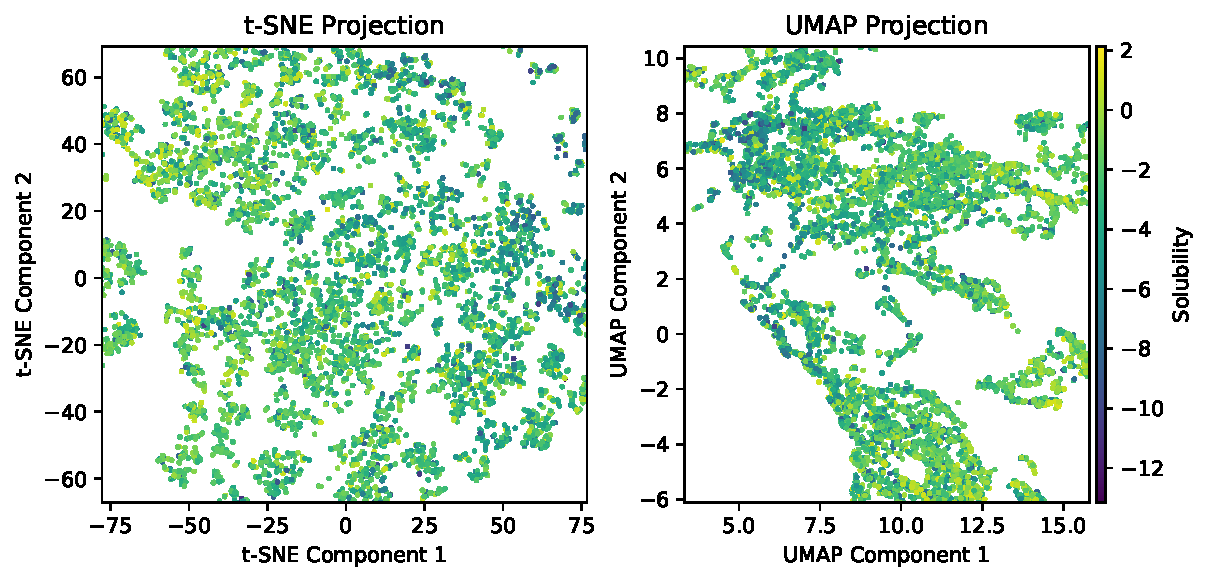
\includegraphics[width=1\textwidth]{solubility.pdf}
        \caption{2D projection of the embedding vectors with solubility.}
        \label{fig:solubility}
\end{figure}

\subsection{Training}

Following our architecture design, the model can be trained on two tasks. The first one is a self-supervised task, were node and edge features are denoised and reconstructed. For this, the features were pertrubed by randomly flipping a percentage of the one-hot encoded node and edge features. The encoder then learns to create an information-dense representation in form of the embedding vector, from which the decoder learns to reconstruct the denoised node and edge features. The second task is the supervised task, where the model learns to predict the solubility value from the embedding vector.

As in literature, both tasks are trained simultaneously by combining the losses \cite{cui2025online, wang2022test}. We followed this approach by using a weighted sum of the two losses, where the weight was optimized to $\alpha = 0.3$ for the self-supervised task and $ 1 - \alpha = 0.7$ for the supervised task. The model was trained for 20 epochs with a batch size of 512, using the Adam optimizer with a learning rate of $0.0026$, weight decay of $5 \cot 10^{-6}$, and dropout of $0.3$.

\begin{figure}[htbp]
        \centering
        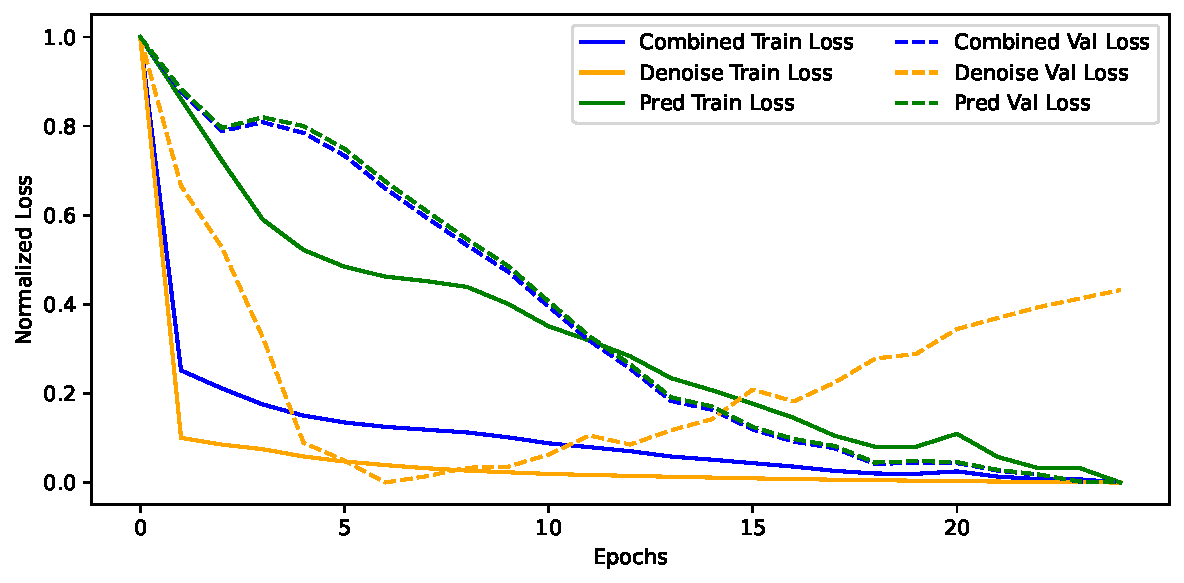
\includegraphics[width=1\textwidth]{loss_plot.pdf}
        \caption{Training and validation losses.}
        \label{fig:loss_plot}
\end{figure}

\subsection{Test-time Adaptation and Prediction}

For TTA, each test sample is processed individually, with the encoder being adapted to the specific molecular structure through a single gradient descent step on the self-supervised loss. The adapted model is then utilized to predict the solubility using the standard prediction head. Following this, the model is set back to its original state, ready for the next test sample. The step size for the gradient descent step was optimized to $2.1 \cdot 10^{-4}$. Doing this, the embedding vector of the test samples should be shifted towards the training set distribution, allowing the model to generalize better. This can be seen in the 2D projections of the embedding vectors in Figure \ref{fig:sets} and \ref{fig:sets_TTA}.

\begin{figure}[htbp]
        \centering
        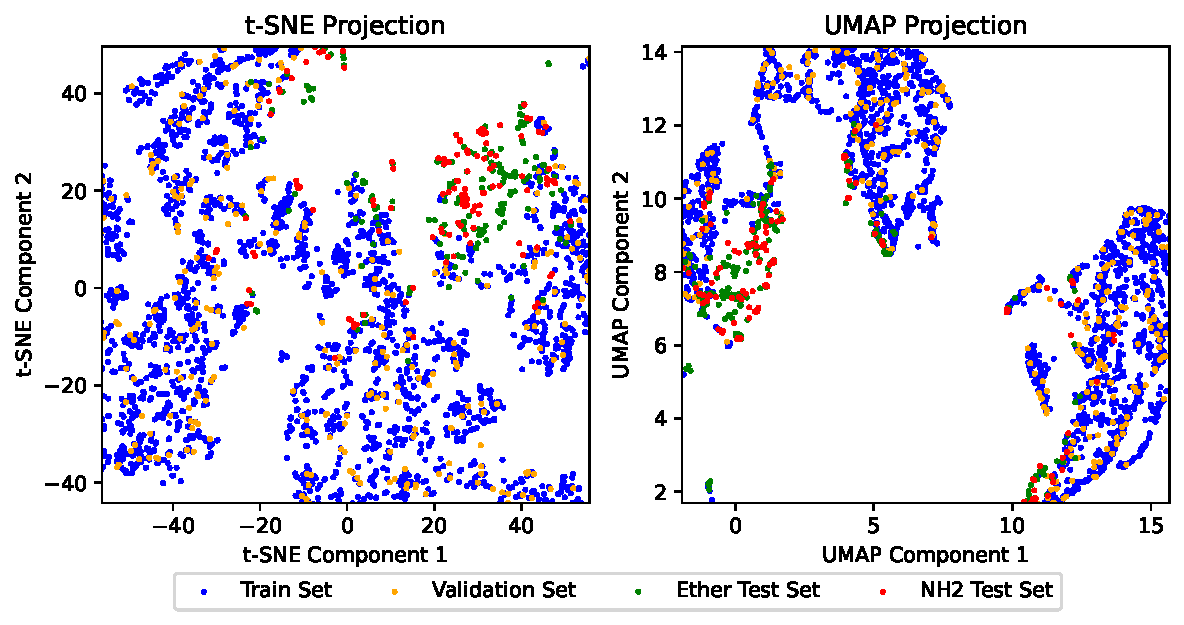
\includegraphics[width=1\textwidth]{sets.pdf}
        \caption{2D projection of the embedding vectors with sets.}
        \label{fig:sets}
\end{figure}

\begin{figure}[htbp]
        \centering
        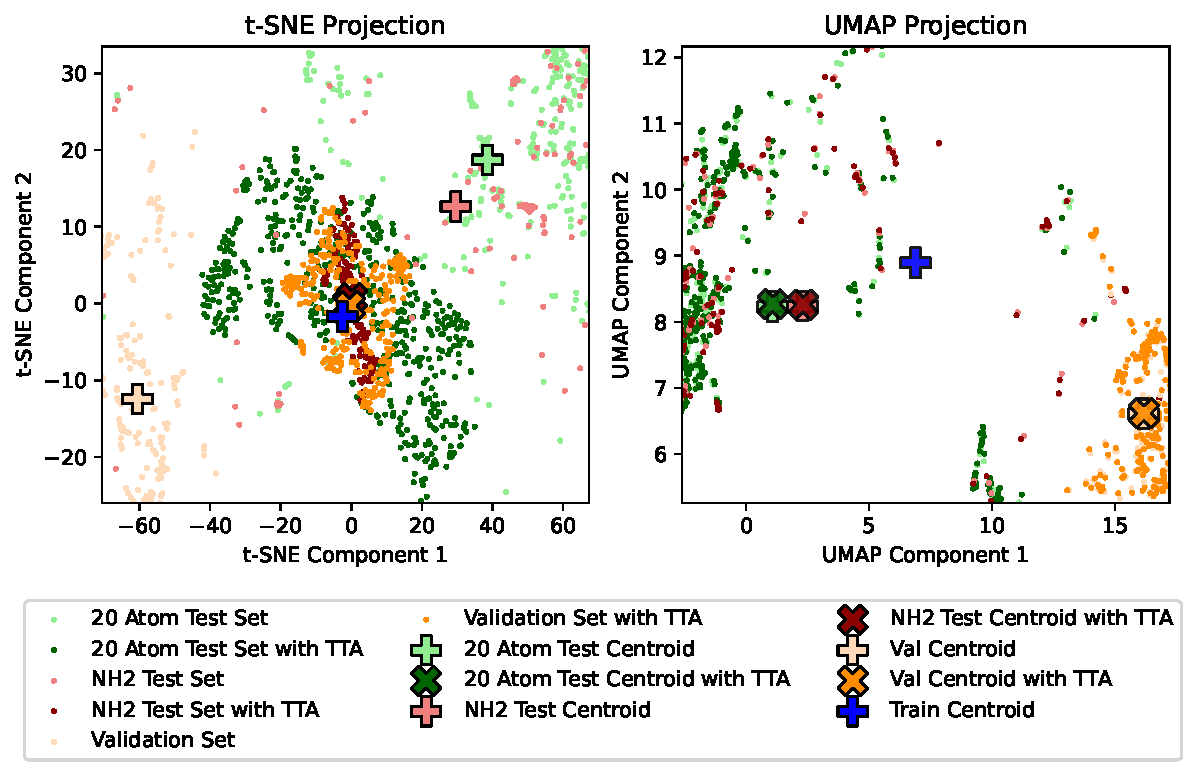
\includegraphics[width=1\textwidth]{sets_TTA.pdf}
        \caption{2D projection of the embedding vectors with set centroids.}
        \label{fig:sets_TTA}
\end{figure}

\section{Results}

\begin{table}[htbp]
        \centering
        \begin{tabular}{@{}lcc@{}}
                \toprule
                \textbf{Model}    & \textbf{Validation RMSE} & \textbf{Test RMSE} \\
                \midrule
                Model without TTA & 1.05                     & 1.41               \\
                Model with TTA    & 1.06                     & 1.41               \\
                Reference Model   & 2.09                     & 2.26               \\
                \bottomrule
        \end{tabular}
        \caption{Performance comparison of different model configurations.}
        \label{tab:results}
\end{table}

As shown in Table \ref{tab:results}, TTA did not improve the performance of the model on the test set, which is suprising, given that the test set centroid clearly shifts towards the training set centroid after TTA, as shown in the 2D projections of the embedding space in Figure \ref{fig:sets_TTA}. Maybe this would work better for other datasets with a larger distribution shift.

For comparison, a reference model trained solely on the prediction task without any self-supervised learning (SSL) was also included. This showed that SSL clearly improves the prediction performance.

\section{Conclusion}

This project applied test-time adaptation to graph neural networks for molecular solubility prediction. While TTA successfully shifted the test set embeddings towards the training distribution, as demonstrated through embedding space visualizations, this did not translate into improved predictive performance on the test set used here.

\bibliographystyle{plain}
\bibliography{references}

\end{document}